\documentclass{report}
\usepackage[T1]{fontenc}
\usepackage[french]{babel}
\usepackage{graphicx}
\usepackage{float}
\usepackage{fullpage}
\usepackage{eso-pic}
\usepackage{listings} %ce package va nous permettre d'encadrer notre code 


\lstset{
  language=SQL,
  basicstyle=\ttfamily,
  numbers=left,
  numberstyle=\tiny,
  keywordstyle = \color{green},
  frame=single,
  breaklines=true,
  columns=fullflexible,
  float, % Utiliser cette option pour permettre le flottement du bloc de code
}


\begin{document}
\listoffigures
\tableofcontents
\chapter{INTRODUCTION}
À travers ce projet, notre objectif a été de nous servir des compétences et connaissances acquises au cours du module de gestion de base de données.\\
Aussi, nous avons choisi d'utiliser le langage JAVA pour créer l'application liée à la base de données, afin de créer une synergie entre les deux modules.\\
Notre application a pour but de reproduire en partie le fonctionnement de l'application de réservation de meublés touristiques: Airbnb.\\
Le fonctionnement d'une telle application étant quelque peu complexe, nous avons fait le choix de ne pas doter notre version de l'ensemble des fonctionnalités disponible sur Airbnb.\\
\chapter{Création du MCD}
Pour créer notre MCD, nous nous sommes servis de \textbf{\emph{mysqlworkbench}}, logiciel qui nous a été présenté lors du module et qui nous permet de créer des diagrammes qui mettent en lumière les différentes connexions entre les tables qui composent notre base de données.\\
De plus, il va nous permettre de convertir ledit diagramme en une requête \textbf{SQL} pour implémenter notre base de données.
\begin{figure}[H] %le H majuscule est hyper important pour que la figure respecte l'emplacement qu'on lui donne !!!
    \begin{center}
        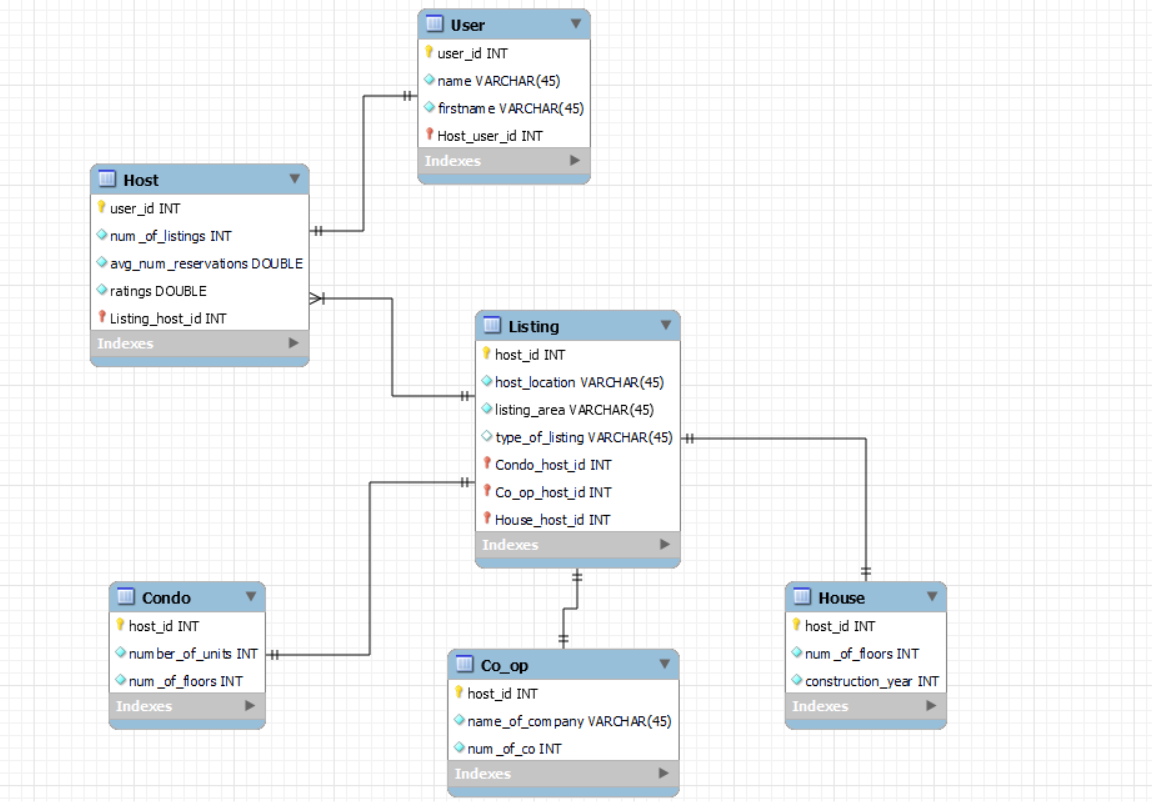
\includegraphics[width=0.6\linewidth]{diagramme.png}
         \caption{Diagramme EER}
    \end{center}
\end{figure}
\newpage 
Ce qui une fois converti en une requête \textbf{SQL} nous donne:
\begin{lstlisting}
    CREATE TABLE IF NOT EXISTS `mydb`.`Condo` (
        `host_id` INT NOT NULL,
        `number_of_units` INT NOT NULL,
        `num_of_floors` INT NOT NULL,
        PRIMARY KEY (`host_id`))
      ENGINE = InnoDB;
    \end{lstlisting}

    \begin{lstlisting}
      -- -----------------------------------------------------
      -- Table `mydb`.`Co_op`
      -- -----------------------------------------------------
      CREATE TABLE IF NOT EXISTS `mydb`.`Co_op` (
        `host_id` INT NOT NULL,
        `name_of_company` VARCHAR(45) NOT NULL,
        `num_of_co` INT NOT NULL,
        PRIMARY KEY (`host_id`))
      ENGINE = InnoDB;
    \end{lstlisting}


    \begin{lstlisting}
      -- -----------------------------------------------------
      -- Table `mydb`.`House`
      -- -----------------------------------------------------
      CREATE TABLE IF NOT EXISTS `mydb`.`House` (
        `host_id` INT NOT NULL,
        `num_of_floors` INT NOT NULL,
        `construction_year` INT NOT NULL,
        PRIMARY KEY (`host_id`))
      ENGINE = InnoDB;
    \end{lstlisting}


    \begin{lstlisting}
      -- -----------------------------------------------------
      -- Table `mydb`.`Listing`
      -- -----------------------------------------------------
      CREATE TABLE IF NOT EXISTS `mydb`.`Listing` (
        `host_id` INT NOT NULL,
        `host_location` VARCHAR(45) NOT NULL,
        `listing_area` VARCHAR(45) NOT NULL,
        `type_of_listing` VARCHAR(45) NULL,
        `Condo_host_id` INT NULL,
        `Co_op_host_id` INT NULL,
        `House_host_id` INT NULL,
        PRIMARY KEY (`host_id`, `Condo_host_id`, `Co_op_host_id`, `House_host_id`),
        INDEX `fk_Listing_Condo1_idx` (`Condo_host_id` ASC) VISIBLE,
        INDEX `fk_Listing_Co_op1_idx` (`Co_op_host_id` ASC) VISIBLE,
        INDEX `fk_Listing_House1_idx` (`House_host_id` ASC) VISIBLE,
        CONSTRAINT `fk_Listing_Condo1`
          FOREIGN KEY (`Condo_host_id`)
          REFERENCES `mydb`.`Condo` (`host_id`)
          ON DELETE NO ACTION
          ON UPDATE NO ACTION,
        CONSTRAINT `fk_Listing_Co_op1`
          FOREIGN KEY (`Co_op_host_id`)
          REFERENCES `mydb`.`Co_op` (`host_id`)
          ON DELETE NO ACTION
          ON UPDATE NO ACTION,
        CONSTRAINT `fk_Listing_House1`
          FOREIGN KEY (`House_host_id`)
          REFERENCES `mydb`.`House` (`host_id`)
          ON DELETE NO ACTION
          ON UPDATE NO ACTION)
      ENGINE = InnoDB;
    \end{lstlisting}

    \begin{lstlisting}
      -- -----------------------------------------------------
      -- Table `mydb`.`Host`
      -- -----------------------------------------------------
      CREATE TABLE IF NOT EXISTS `mydb`.`Host` (
        `user_id` INT NOT NULL,
        `num_of_listings` INT NOT NULL,
        `avg_num_reservations` DOUBLE NOT NULL,
        `ratings` DOUBLE NOT NULL,
        `Listing_host_id` INT NOT NULL,
        PRIMARY KEY (`user_id`, `Listing_host_id`),
        INDEX `fk_Host_Listing1_idx` (`Listing_host_id` ASC) VISIBLE,
        CONSTRAINT `fk_Host_Listing1`
          FOREIGN KEY (`Listing_host_id`)
          REFERENCES `mydb`.`Listing` (`host_id`)
          ON DELETE NO ACTION
          ON UPDATE NO ACTION)
      ENGINE = InnoDB;
    \end{lstlisting}

    \begin{lstlisting}
      -- -----------------------------------------------------
      -- Table `mydb`.`User`
      -- -----------------------------------------------------
      CREATE TABLE IF NOT EXISTS `mydb`.`User` (
        `user_id` INT NOT NULL AUTO_INCREMENT,
        `name` VARCHAR(45) NOT NULL,
        `firstname` VARCHAR(45) NOT NULL,
        `Host_user_id` INT NOT NULL,
        PRIMARY KEY (`user_id`, `Host_user_id`),
        UNIQUE INDEX `user_id_UNIQUE` (`user_id` ASC) VISIBLE,
        INDEX `fk_User_Host_idx` (`Host_user_id` ASC) VISIBLE,
        CONSTRAINT `fk_User_Host`
          FOREIGN KEY (`Host_user_id`)
          REFERENCES `mydb`.`Host` (`user_id`)
          ON DELETE NO ACTION
          ON UPDATE NO ACTION)
      ENGINE = InnoDB;
    \end{lstlisting}
\chapter{Implementation du code en JAVA}
\end{document}
